\documentclass[11pt]{article}

% ---------- Packages ----------
\usepackage[a4paper,margin=1in]{geometry}
\usepackage{amsmath, amssymb}
\usepackage{graphicx}
\usepackage{xcolor}
\usepackage{titlesec}
\usepackage{fancyhdr}
\usepackage{hyperref}
\usepackage{tikz} % For diagrams
\usetikzlibrary{automata, positioning}

% ---------- Styling ----------
\definecolor{coolblue}{RGB}{30, 90, 160}
\definecolor{softgray}{RGB}{240,240,240}

\titleformat{\section}
  {\Large\bfseries\color{coolblue}}
  {\thesection}{1em}{}

\pagestyle{fancy}
\fancyhf{}
\fancyfoot[C]{\thepage}
\fancyhead[L]{\textit{A Very Cool \LaTeX\ Document}}
\fancyhead[R]{\today}

% ---------- Document ----------
\begin{document}

\begin{center}
    {\Huge\bfseries\color{coolblue} A Super Cool \LaTeX\ Document}\\[0.5em]
    {\large Written like a professional, compiled like magic $\star$}\\[1em]
    \rule{0.8\textwidth}{0.5pt}
\end{center}

\vspace{1em}

\section*{Why \LaTeX\ Is Awesome}

\LaTeX\ lets you focus on \textbf{ideas}, not formatting.  
Everything stays clean, consistent, and professional — even for long documents.

\begin{itemize}
    \item Perfect mathematical typesetting
    \item Automatic numbering and references
    \item No formatting chaos
\end{itemize}

\section*{Some Fancy Math}

Here’s a famous equation, rendered beautifully:

\[
    e^{i\pi} + 1 = 0
\]

And something a bit more serious:

\[
    \nabla \cdot \vec{E} = \frac{\rho}{\varepsilon_0}
\]

---

\section*{Theory of Automata: DFA Example}

Here’s a simple **Deterministic Finite Automaton (DFA)** that accepts strings over $\{0,1\}$ ending in `01`.

\begin{center}
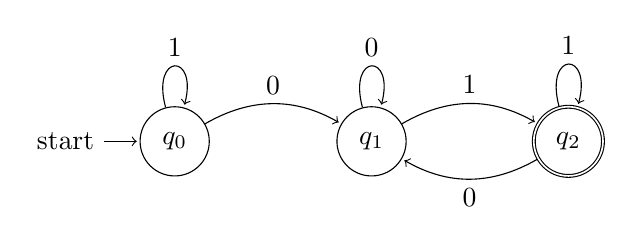
\begin{tikzpicture}[shorten >=1pt, node distance=2.5cm, on grid, auto]
   \node[state, initial] (q0)   {$q_0$};
   \node[state] (q1) [right=of q0] {$q_1$};
   \node[state, accepting] (q2) [right=of q1] {$q_2$};

   \path[->]
    (q0) edge [bend left] node {0} (q1)
         edge [loop above] node {1} ()
    (q1) edge [bend left] node {1} (q2)
         edge [loop above] node {0} ()
    (q2) edge [bend left] node {0} (q1)
         edge [loop above] node {1} ();
\end{tikzpicture}
\end{center}

- $q_0$ = start state  
- $q_2$ = accepting state  
- Accepts strings like `01`, `101`, `001`, etc.

---

\section*{A Highlighted Insight}

\colorbox{softgray}{
\parbox{0.95\textwidth}{
\textbf{Pro tip:}  
Once you stop fighting \LaTeX\ and let it handle structure and layout,  
writing technical documents becomes efficient and reliable.
}}
\vspace{1em}

\section*{Links and References}

Clickable links work out of the box, for example:  
\href{https://www.latex-project.org}{The \LaTeX\ Project Website}

\section*{Final Words}

This document demonstrates:
\begin{enumerate}
    \item Reliable compilation
    \item Professional layout
    \item Scalability to large projects
\end{enumerate}

\begin{center}
    \Large\color{coolblue}
    Welcome to the world of \LaTeX\ $\star$
\end{center}

\end{document}
